\question{}

จากกราฟที่กำหนดให้ดังรูปทางด้าน\ifpageodd{ขวา}{ซ้าย}มือ ข้อใดต่อไปนี้เป็นลำดับของ node ที่\uline{เป็นไปได้}จากการใช้อัลกอริทึม 
Breadth-first search เพื่อ traverse กราฟนี้
\marginnote[-\baselineskip]{%
    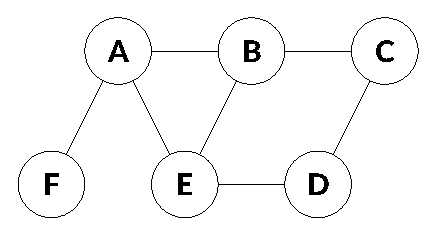
\includegraphics[width=0.98\linewidth]{figures/quickfire_north_audition_validbfs.eps}
}

\begin{multicols}{5}
    \begin{enumerate}[label={$\Circle$}]
        \item \verb|ABCDEF|
        \item \verb|EABDFC|
        \item \verb|BEADCF|
        \item \verb|EABDCF|
        \item \verb|FAEDBC|
    \end{enumerate}
\end{multicols}
